\documentclass{adsdoc}

\newcommand{\doctitle}{Variante en EDH Commander : les rôles cachés « Shogun »}

\title{
    \vspace*{-1cm}
    Variante EDH Commander : les rôles « Shogun »\\
    \Large{Ajoutez des rôles cachés à vos parties d'EDH Commander, pour plus de fun et de variété !}\\
    {
        \large
    \vspace*{0.2cm}
    -- \textbf{Nombre de joueurs :} 4 à 6 joueurs (idéalement 5) \\
    -- \textbf{Durée d'une partie :} plus rapide qu'une partie d'EDH à 5, 1H à 1H30 \\
    -- \textbf{Matériel requis :} un petit paquet des 5 cartes « rôle caché Shogun » fourni, et une carte d'explication, en plus de vos decks d'EDH préférés
    }
}
\date{}

\begin{document}

\maketitle
\thispagestyle{fancy}

\vspace*{-1.5cm}

\noindent


\begin{minipage}[t]{0.40\textwidth}
\vspace{0pt}
\hfill
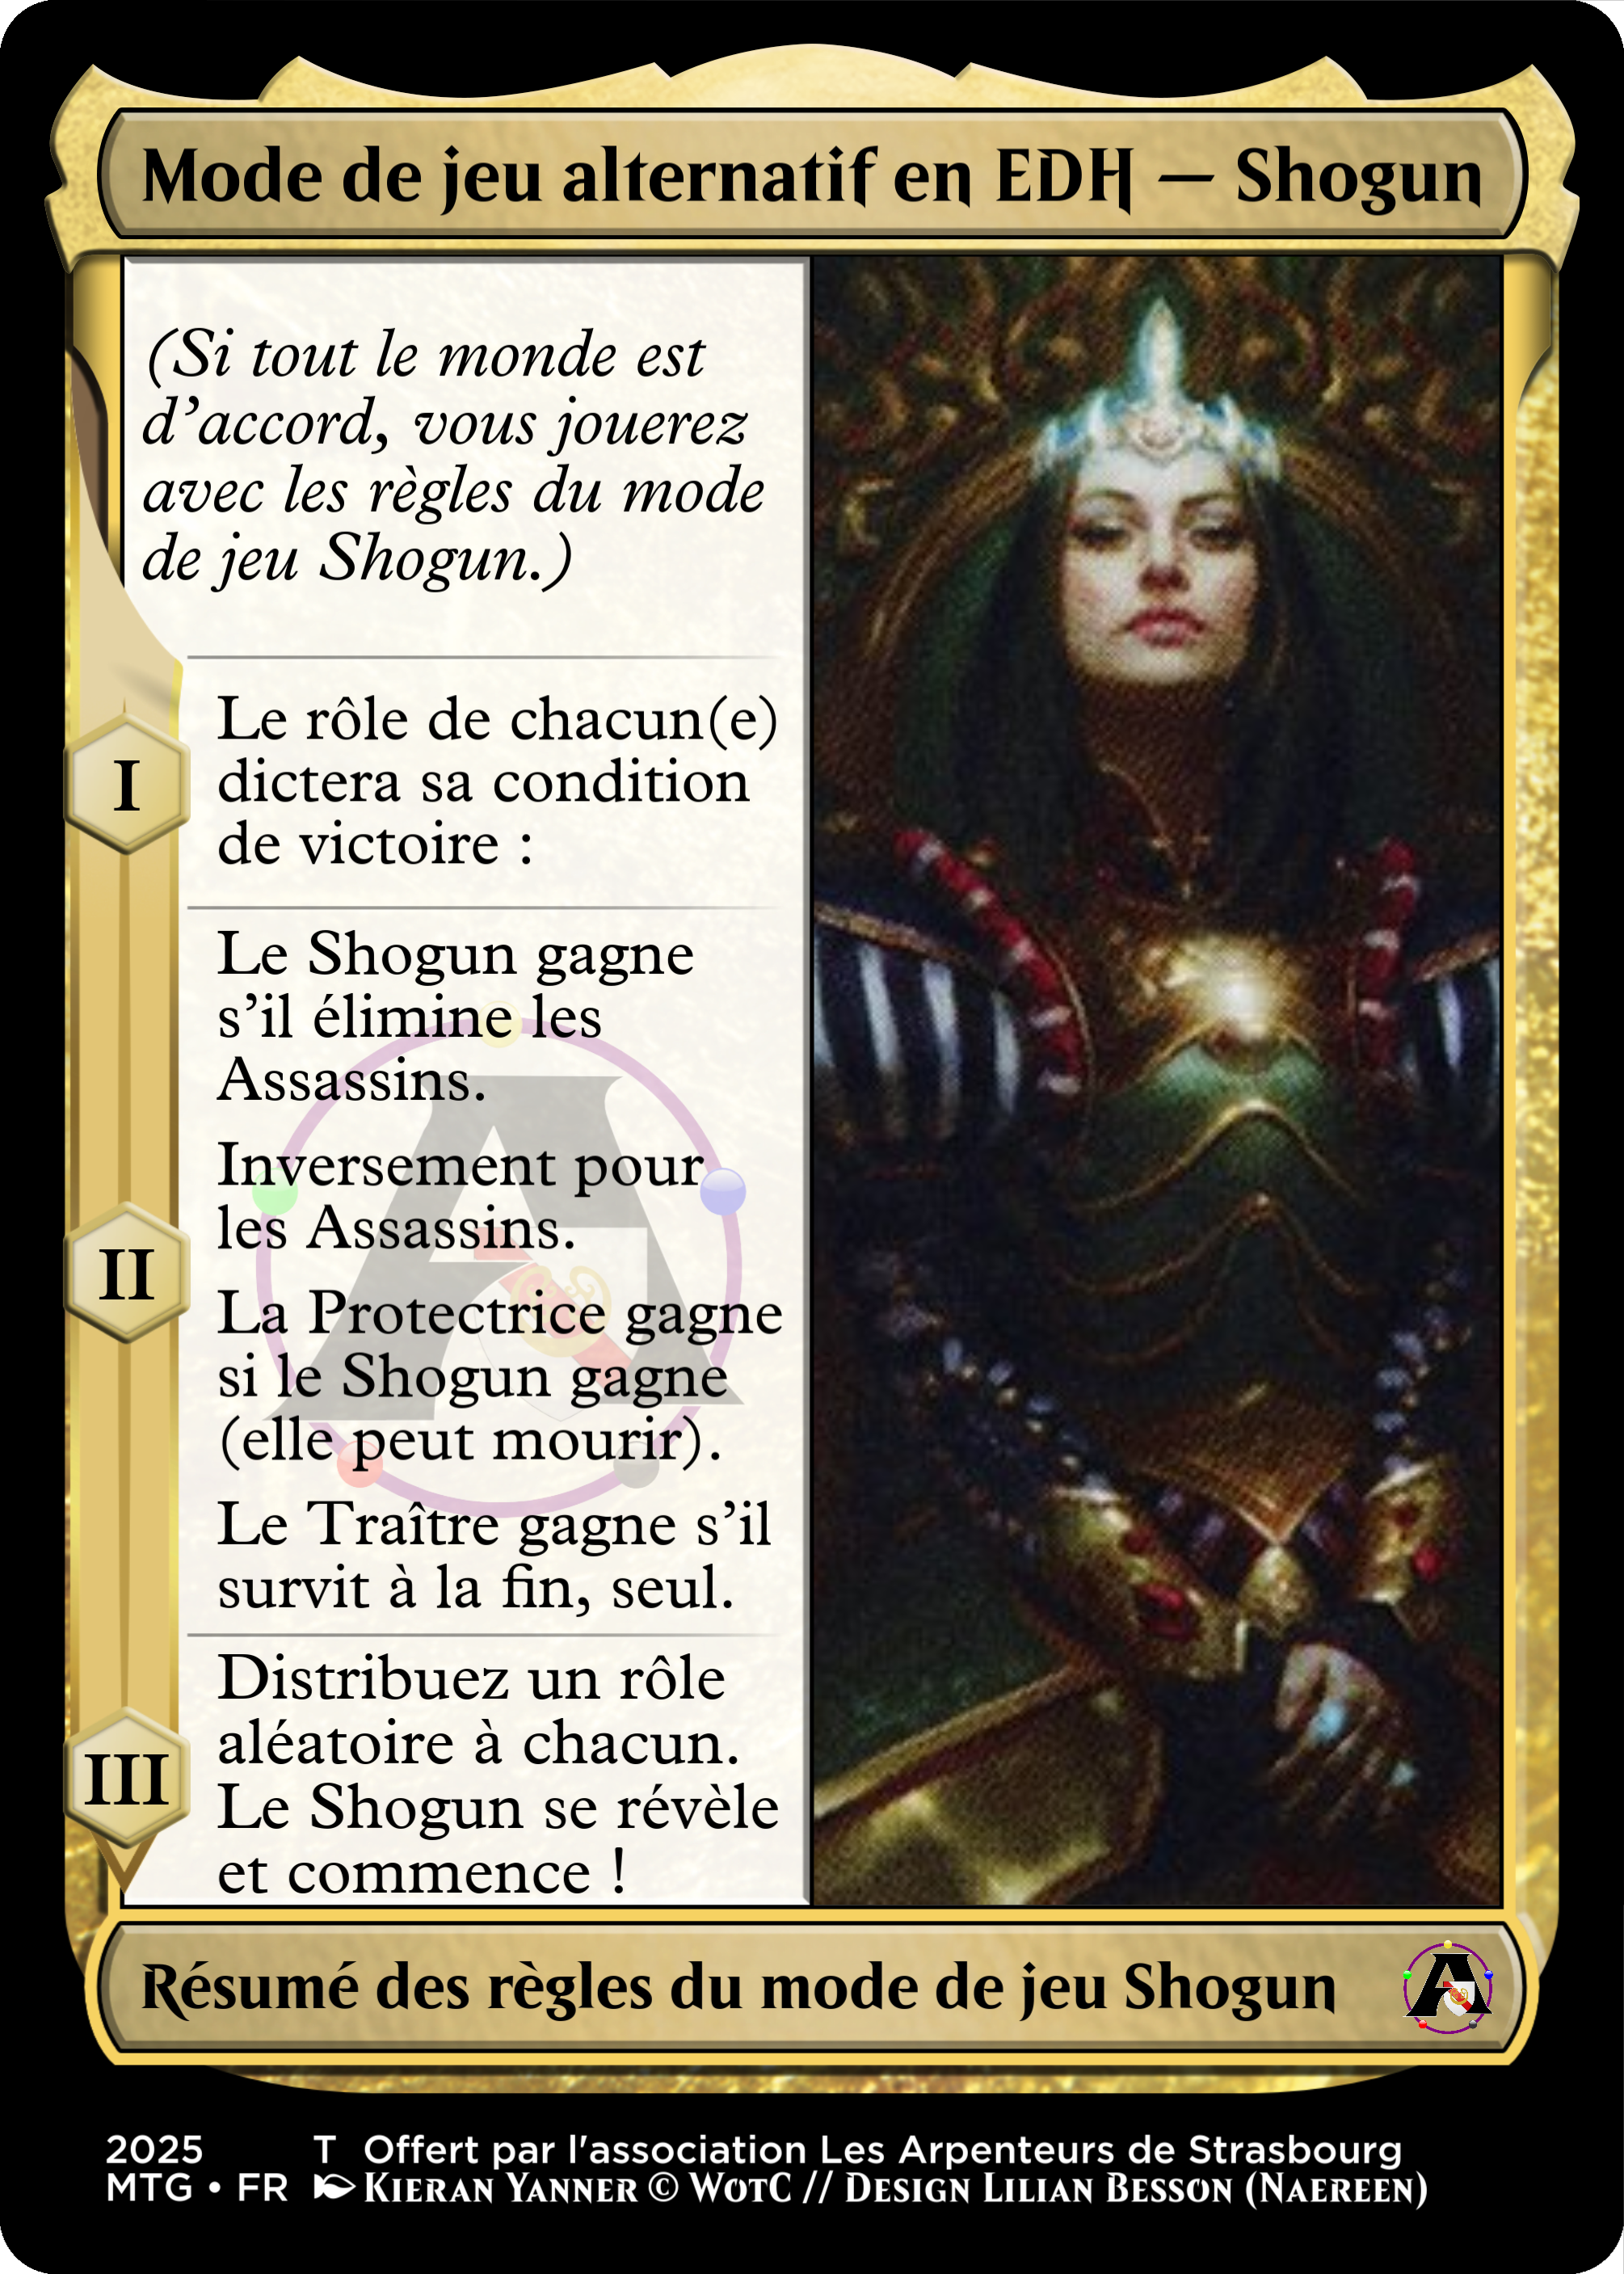
\includegraphics[width=\linewidth]{cartes-pour-le-shogun/explications.png}
\end{minipage}\hfill
\begin{minipage}[t]{0.05\textwidth}
    \vspace{0pt}
\end{minipage}\hfill
\begin{minipage}[t]{0.55\textwidth}
\vspace{0pt}
\begin{itemize}
    \item
    La variante \textbf{Shogun} ajoute une dose de bluff et de politique à vos parties de \textbf{Magic: The Gathering} au format EDH, grâce à un rôle caché reçu en début de partie.
    \item
    Ce rôle caché spécifie votre condition de victoire.
    \item
    Cette variante s'inspire du jeu de cartes \emph{Bang!} ou de jeux de rôles cachés.
    \item
    En France, c'est le « Shogun » et en anglais c'est le « Kingdom ».
    \item
    Voici mes règles de la variante « Shogun » :
\end{itemize}
\end{minipage}

\subsection*{Distribution initiale des rôles « Shogun »}

\begin{itemize}
    \item Choisissez d'abord le niveau de votre table, puis chaque personne choisit son deck, comme dans une partie standard.
    \item \textbf{Distribution initiale des cartes ``Shogun''} : chaque joueur reçoit une carte Shogun, aléatoirement distribuée depuis les cinq rôles disponibles.
        \begin{itemize}
            \item Si vous êtes quatre, distribuez : un Shogun, deux Assassins, un Traître (pas de Gardienne).
            \item \textbf{Si vous êtes cinq, c'est idéal !} Distribuez : un Shogun, une Gardienne, deux Assassins, un Traître.
            \item Si vous êtes six (déconseillé, c'est dur et trop long), distribuez : un Shogun, une Gardienne, deux Assassins, deux Traîtres.
        \end{itemize}
\end{itemize}

\newpage

\subsection*{Règles des rôles « Shogun »}

\begin{itemize}
    \item \textbf{Rôle du Shogun} (1 max) : votre objectif est d'être le dernier joueur en vie. Vous êtes connu de tous les joueurs. Vous commencez à 50 PV et vous commencez la partie.
    \item \textbf{Rôle de la Gardienne} (1 max) : votre objectif est de protéger le Shogun. Si le Shogun meurt, vous perdez également. Vous n'êtes initialement connue de personne. Lorsque vous choisissez de vous révéler, vous gagnez 10 PV et le Shogun aussi.
    \item \textbf{Rôle des Assassins} (2 max) : votre objectif est de tuer le Shogun. Vous n'êtes initialement connu de personne. Vous pouvez vous révéler, et si les deux Assassins sont révélés, ils ne comptent plus comme des Adversaires (pour les sorts et capacités qui ciblent ou se déclenchent pour les adversaires). Si le Shogun meurt, vous gagnez la partie (les deux Assassins peuvent gagner mutuellement, bravo à eux !).
    \item \textbf{Rôle du Traître} (2 max) : votre objectif est de tuer le Shogun, sans que les Assassins gagnent, donc après les avoir éliminés. Vous n'êtes initialement connu de personne. Si le Shogun perd sans que les Assassins soient encore en vie, vous gagnez la partie. C'est évidemment le rôle le plus difficile.
\end{itemize}

\subsection*{Les cartes de rôle « Shogun »}

Je propose ces cartes de rôle, à imprimer et découper, pour jouer à cette variante.

\hfill{}

\begin{center}
    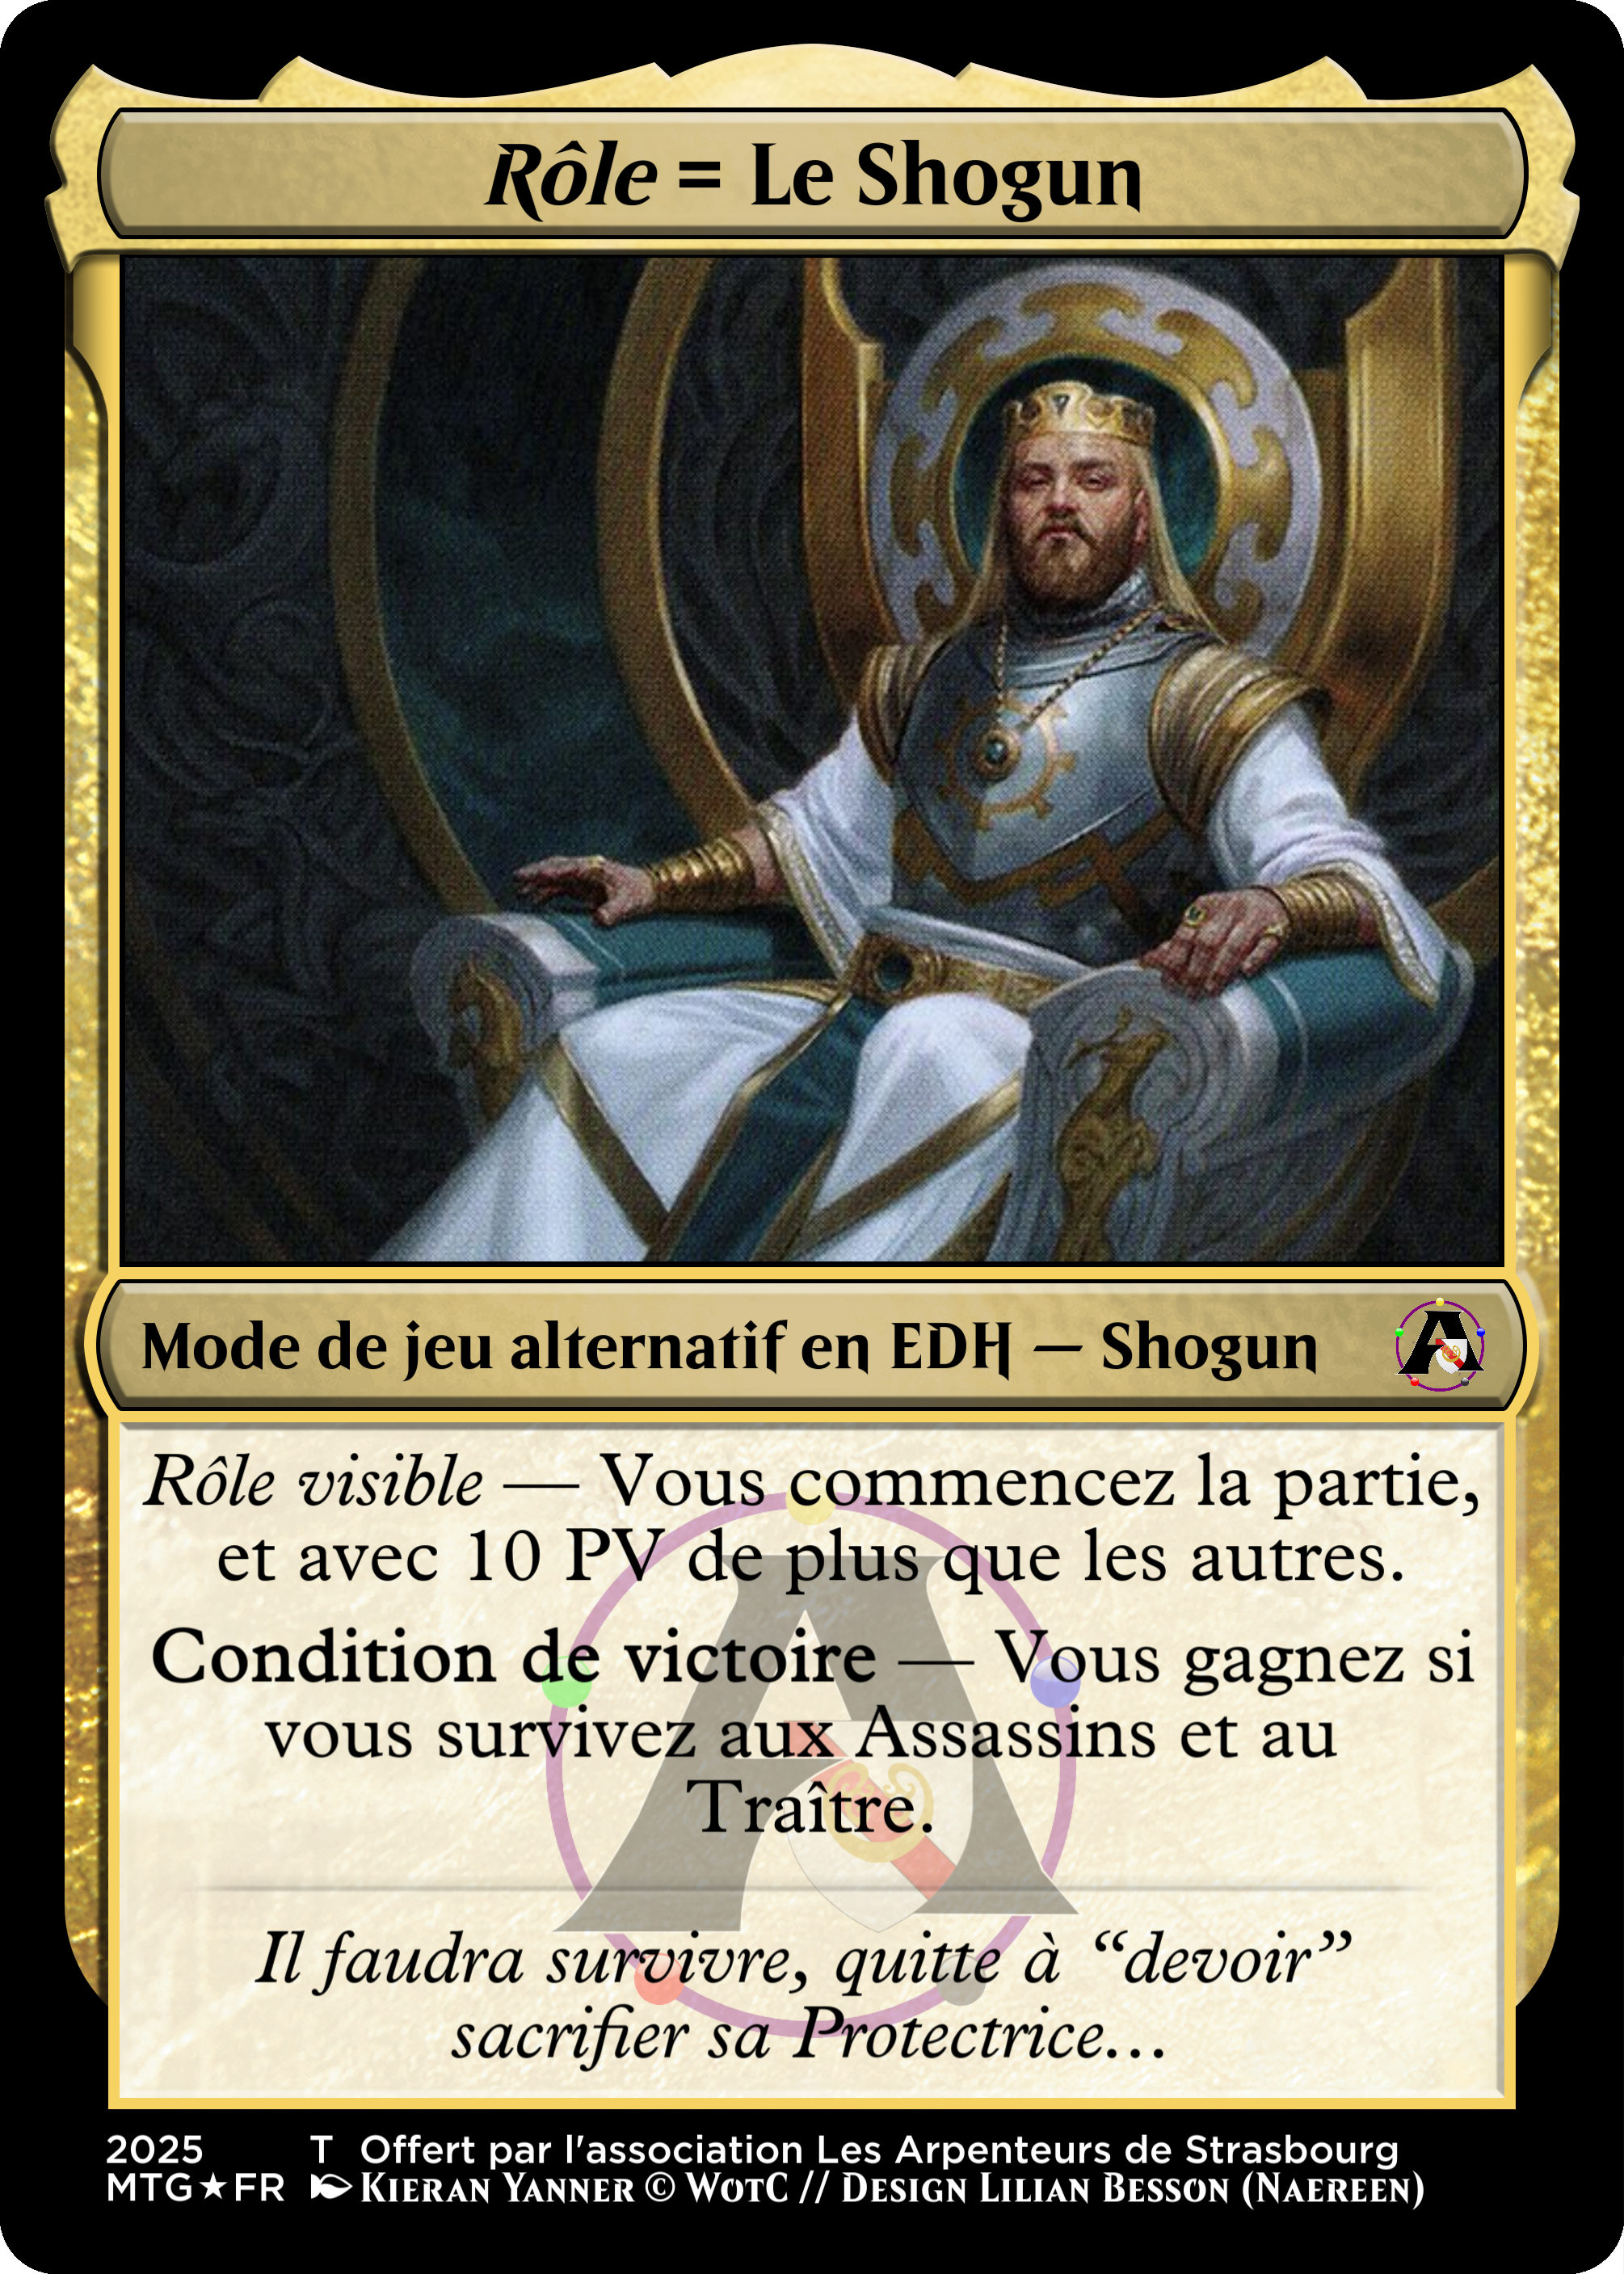
\includegraphics[width=0.21\linewidth]{cartes-pour-le-shogun/shogun.png}
    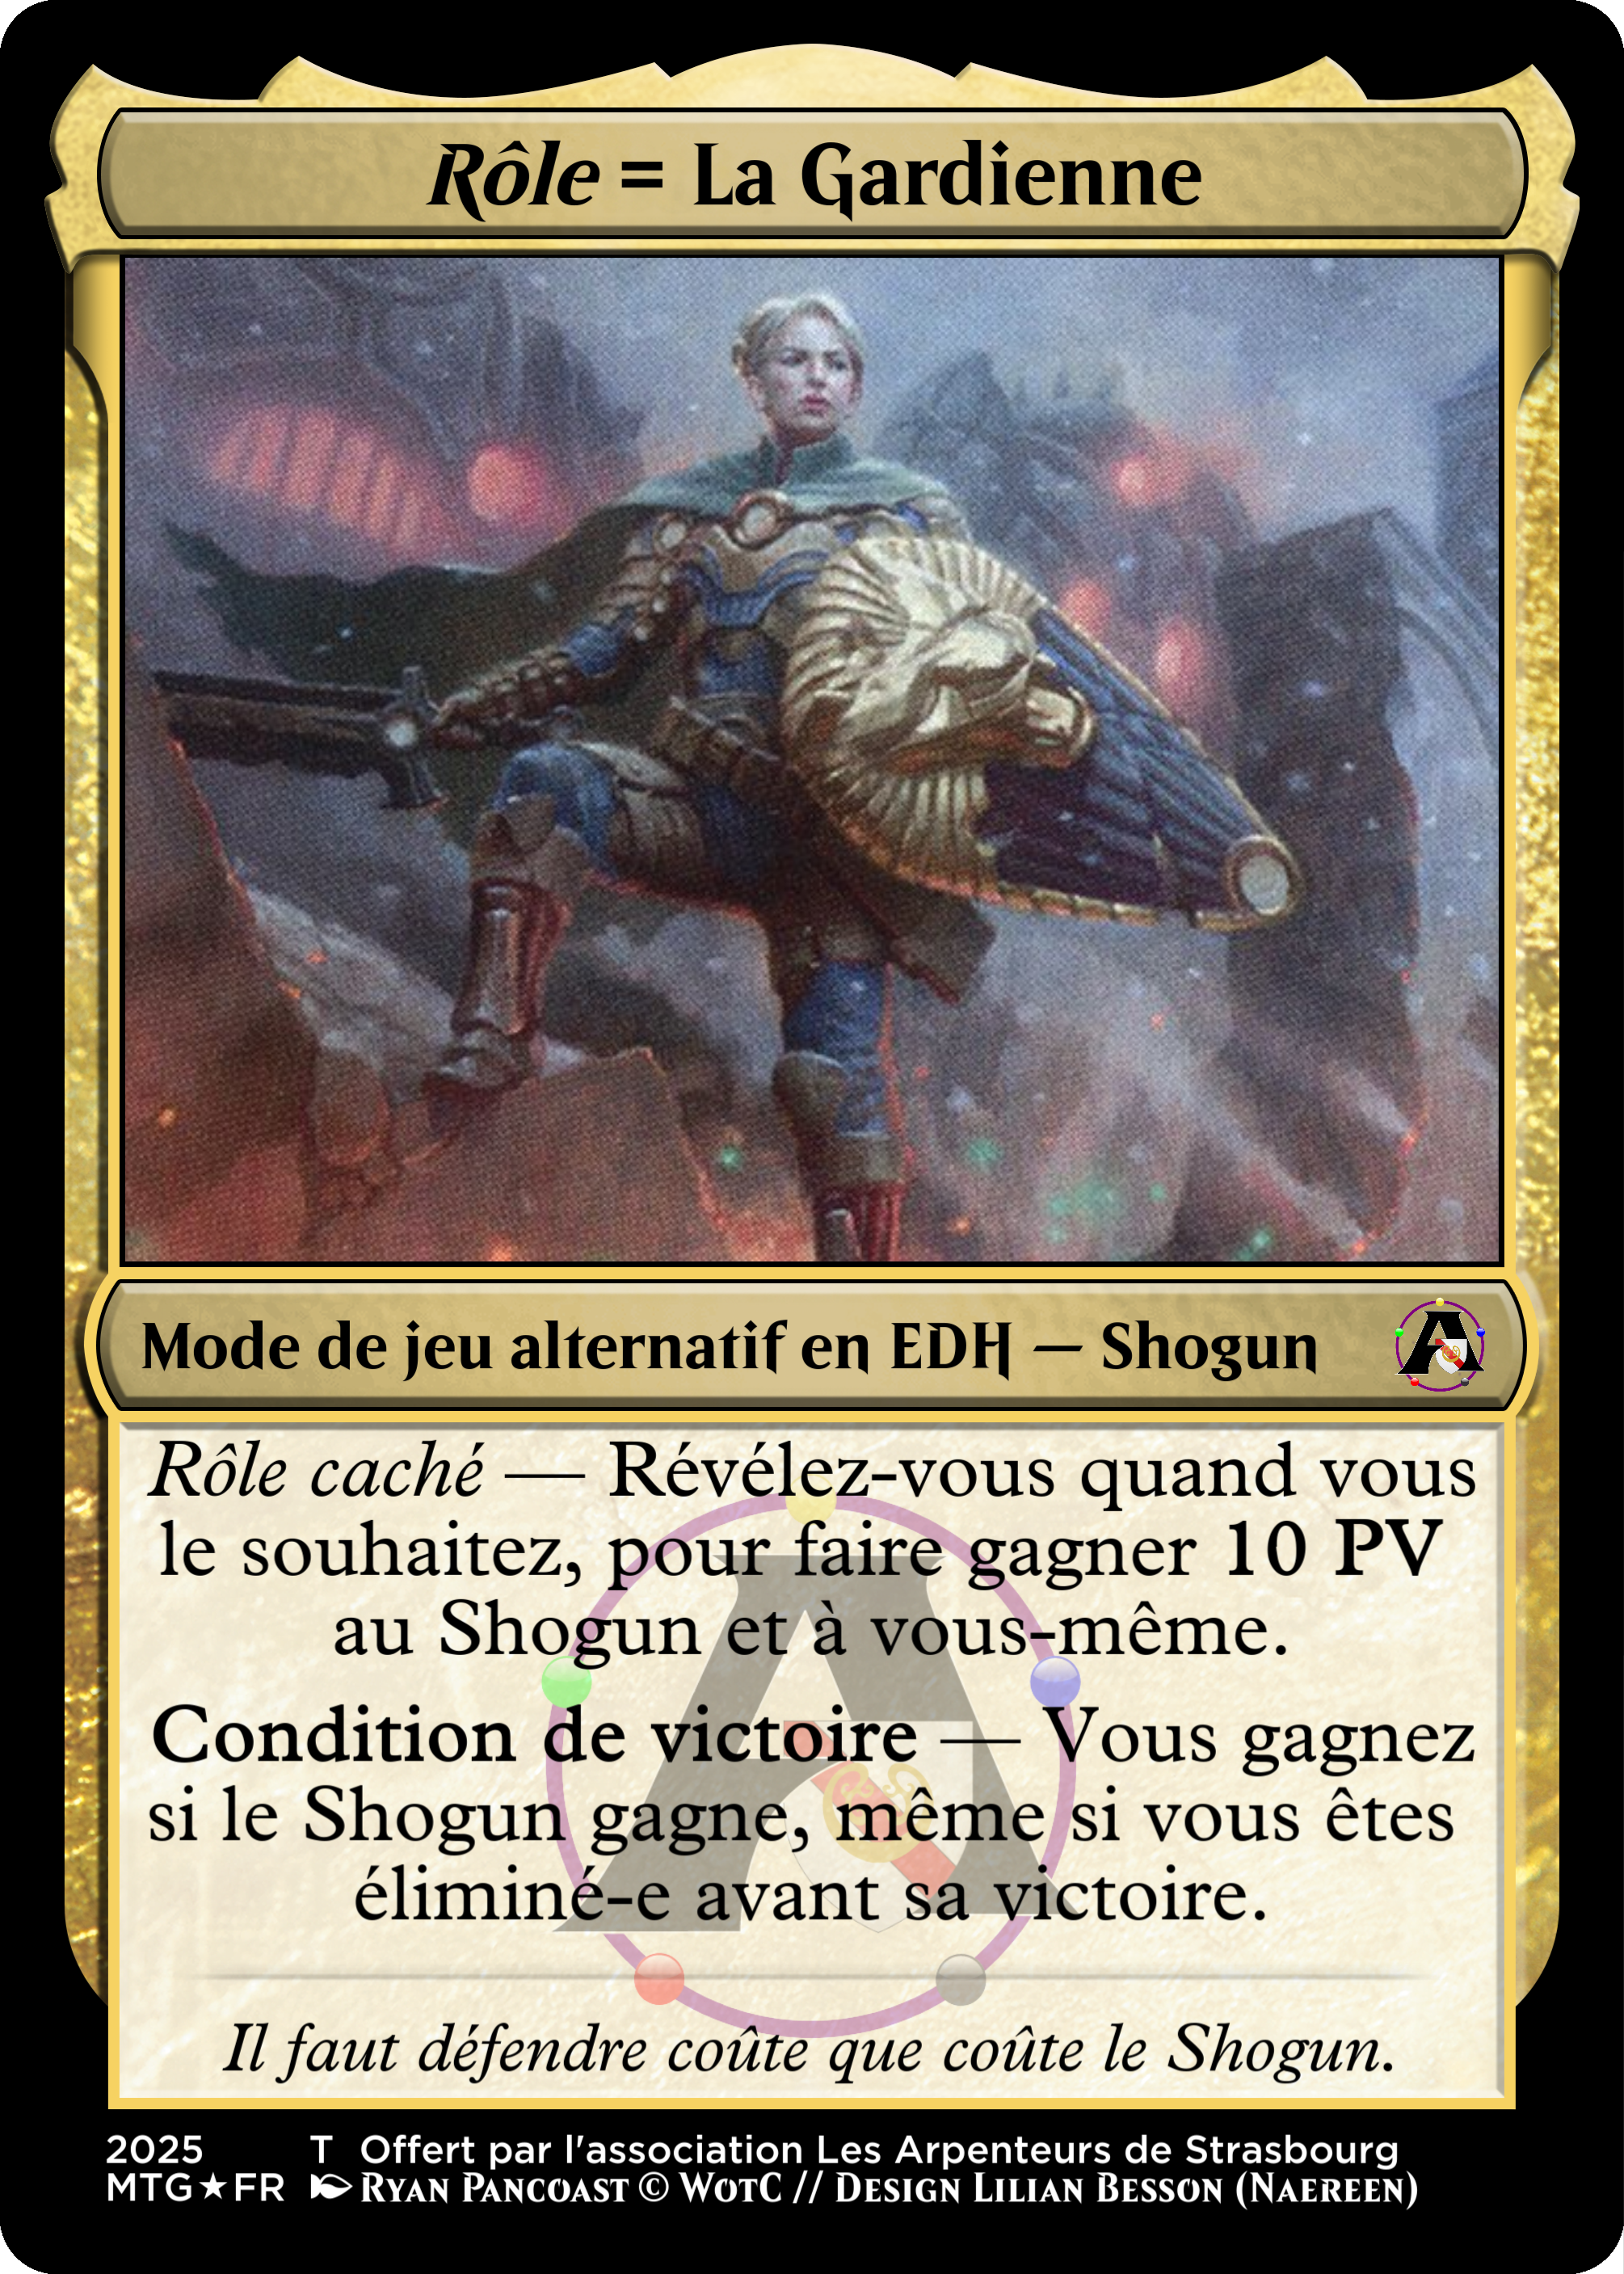
\includegraphics[width=0.21\linewidth]{cartes-pour-le-shogun/guardienne.png}
    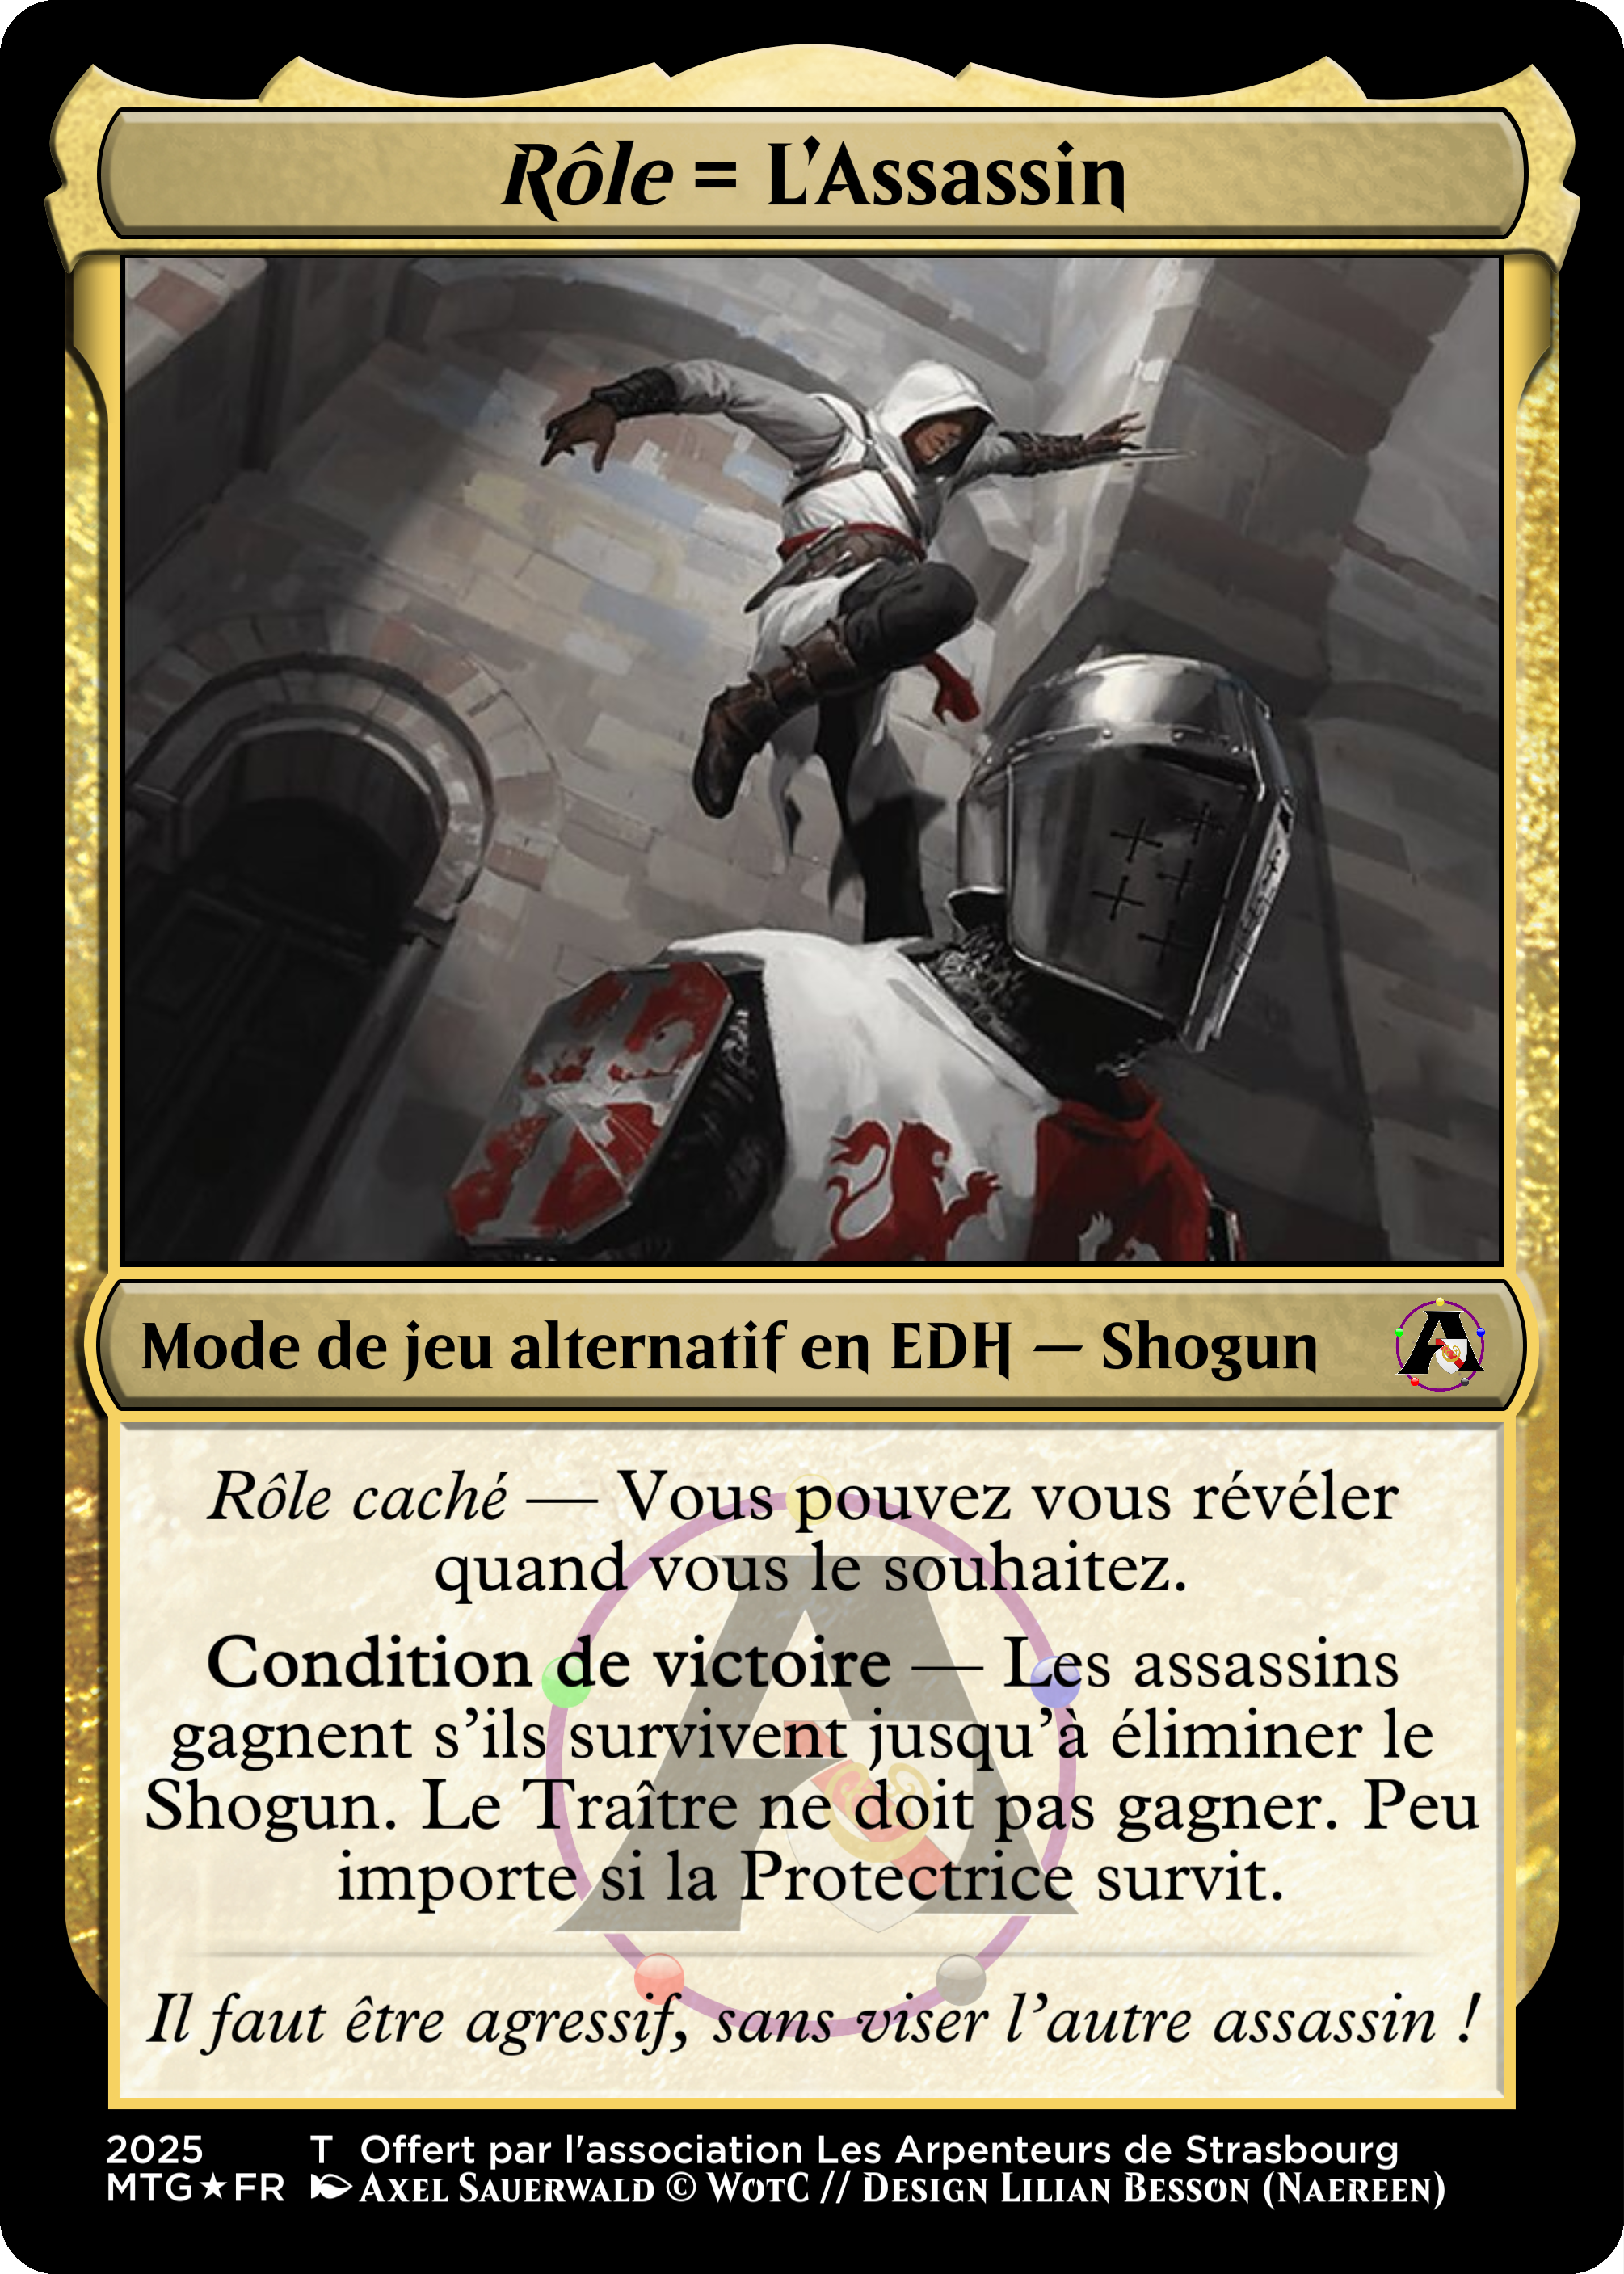
\includegraphics[width=0.21\linewidth]{cartes-pour-le-shogun/assassin1.png}
    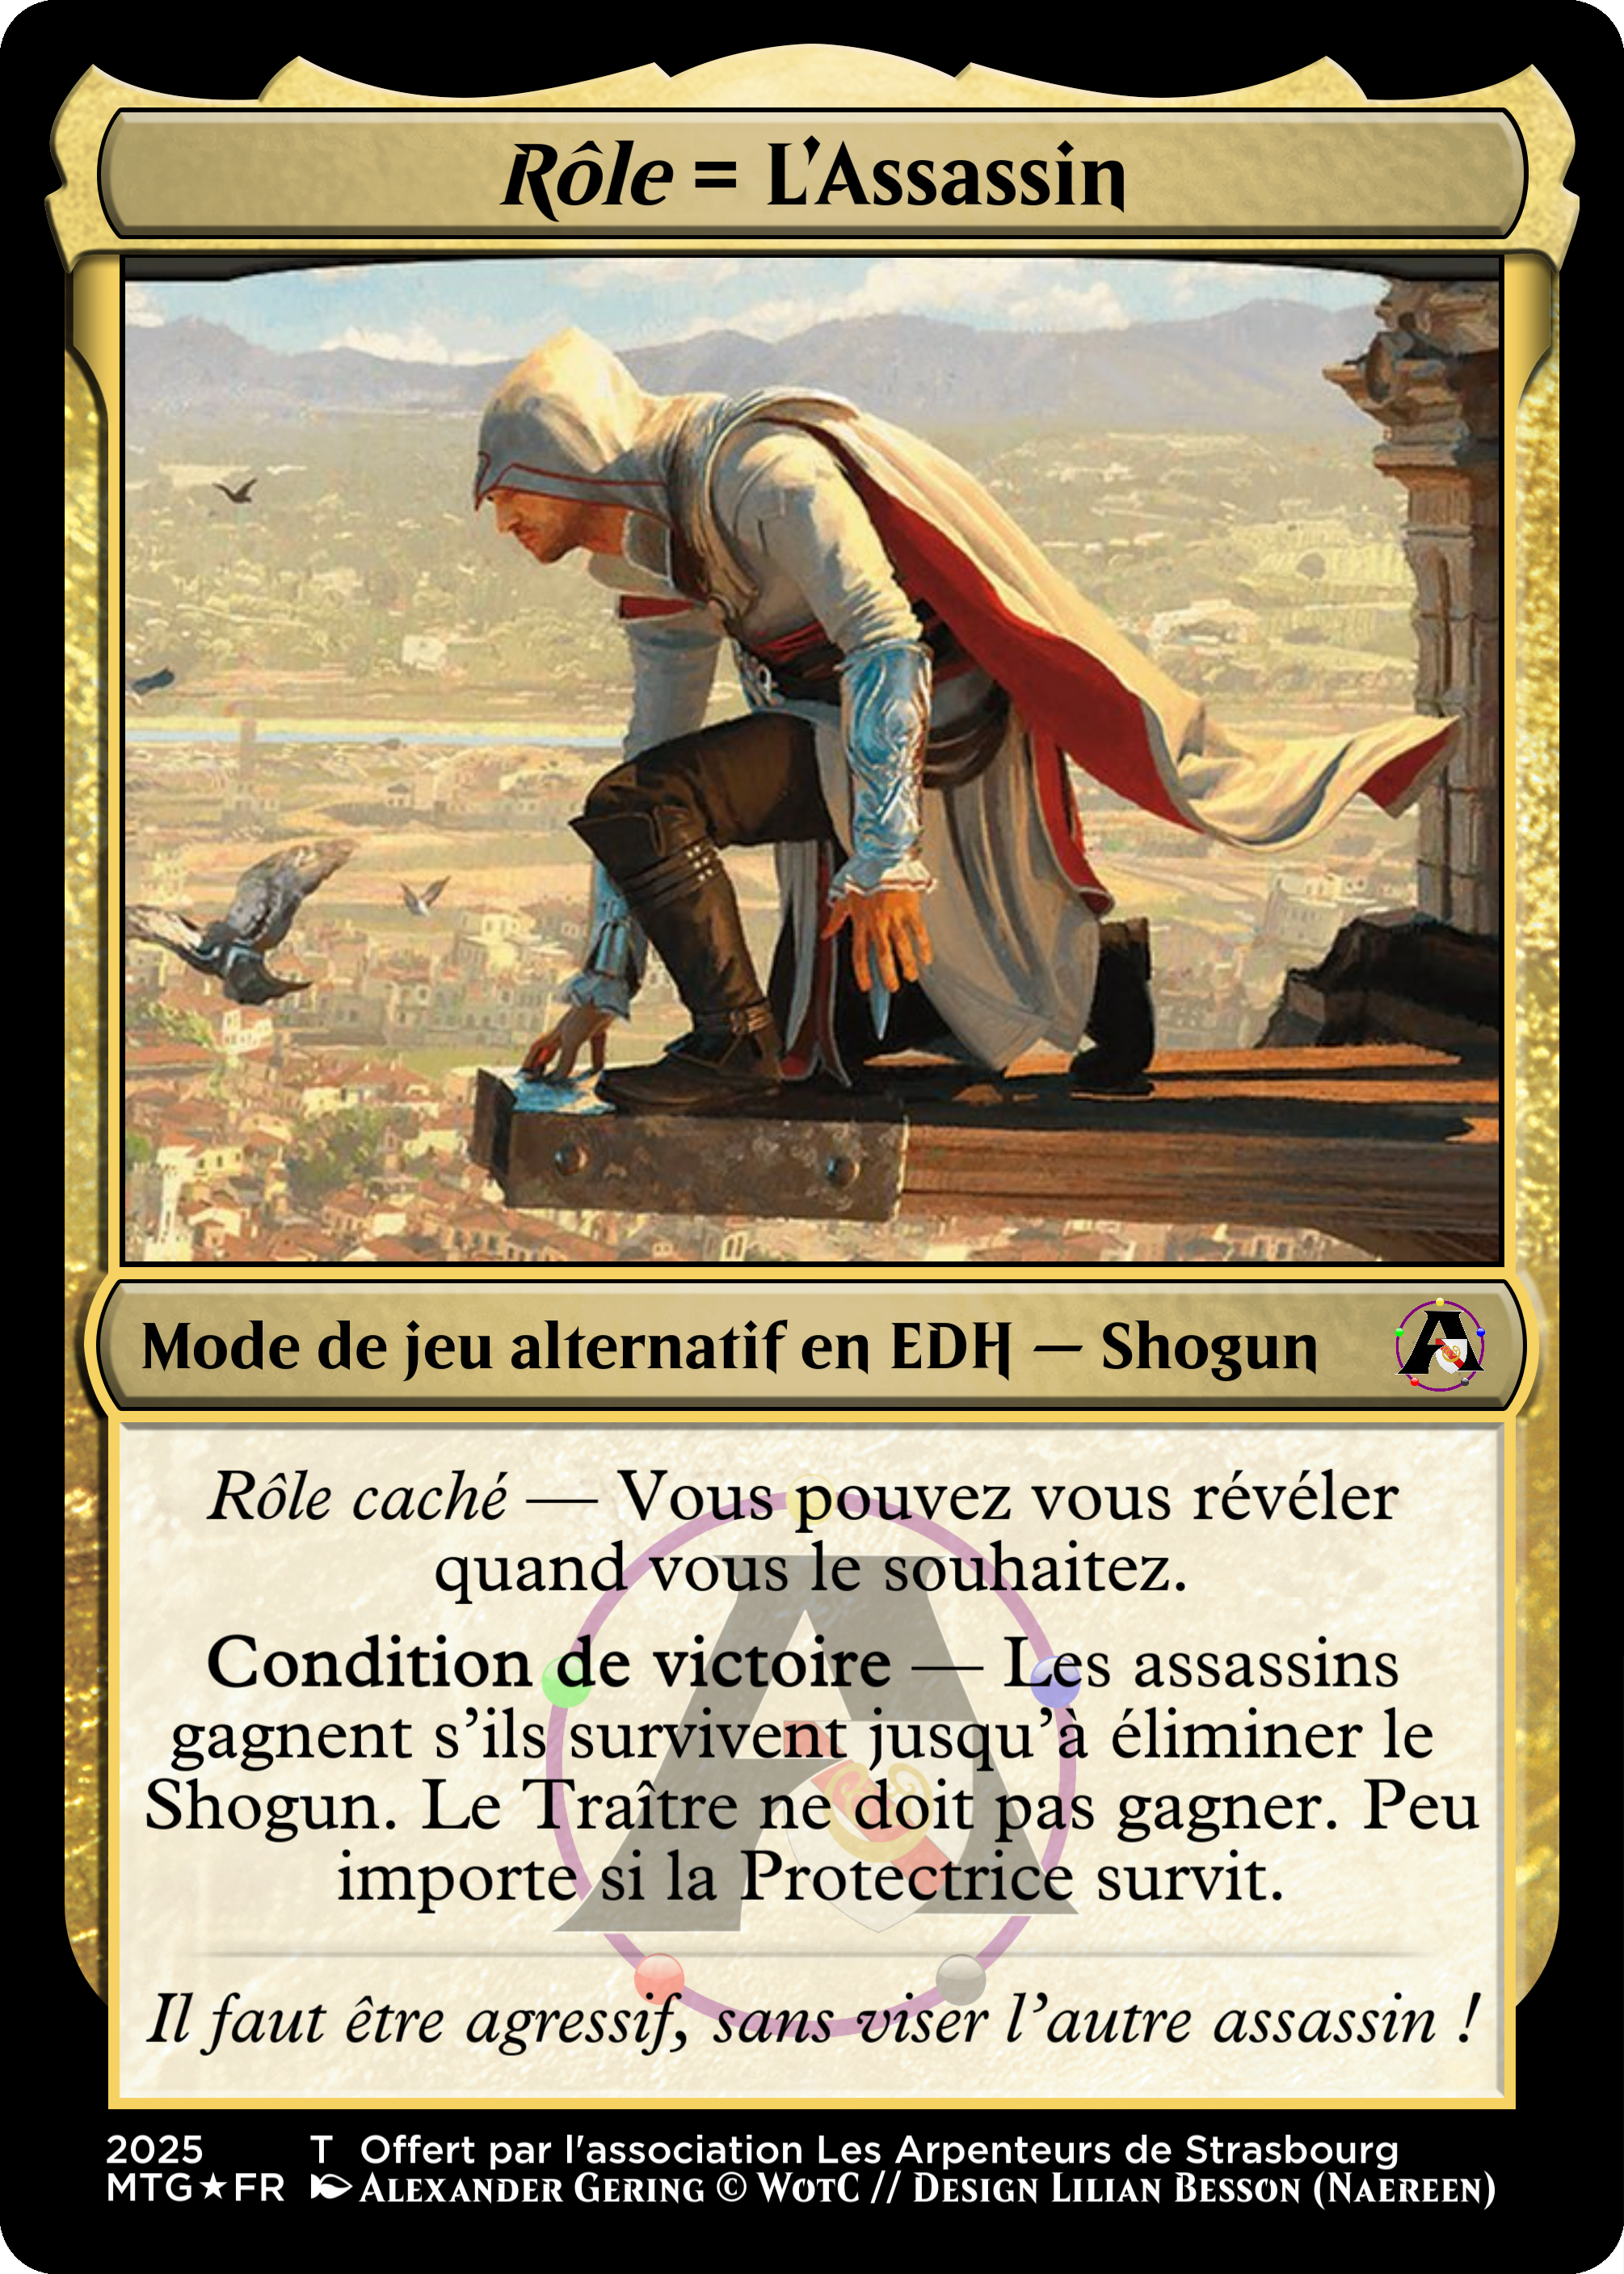
\includegraphics[width=0.21\linewidth]{cartes-pour-le-shogun/assassin2.png}
    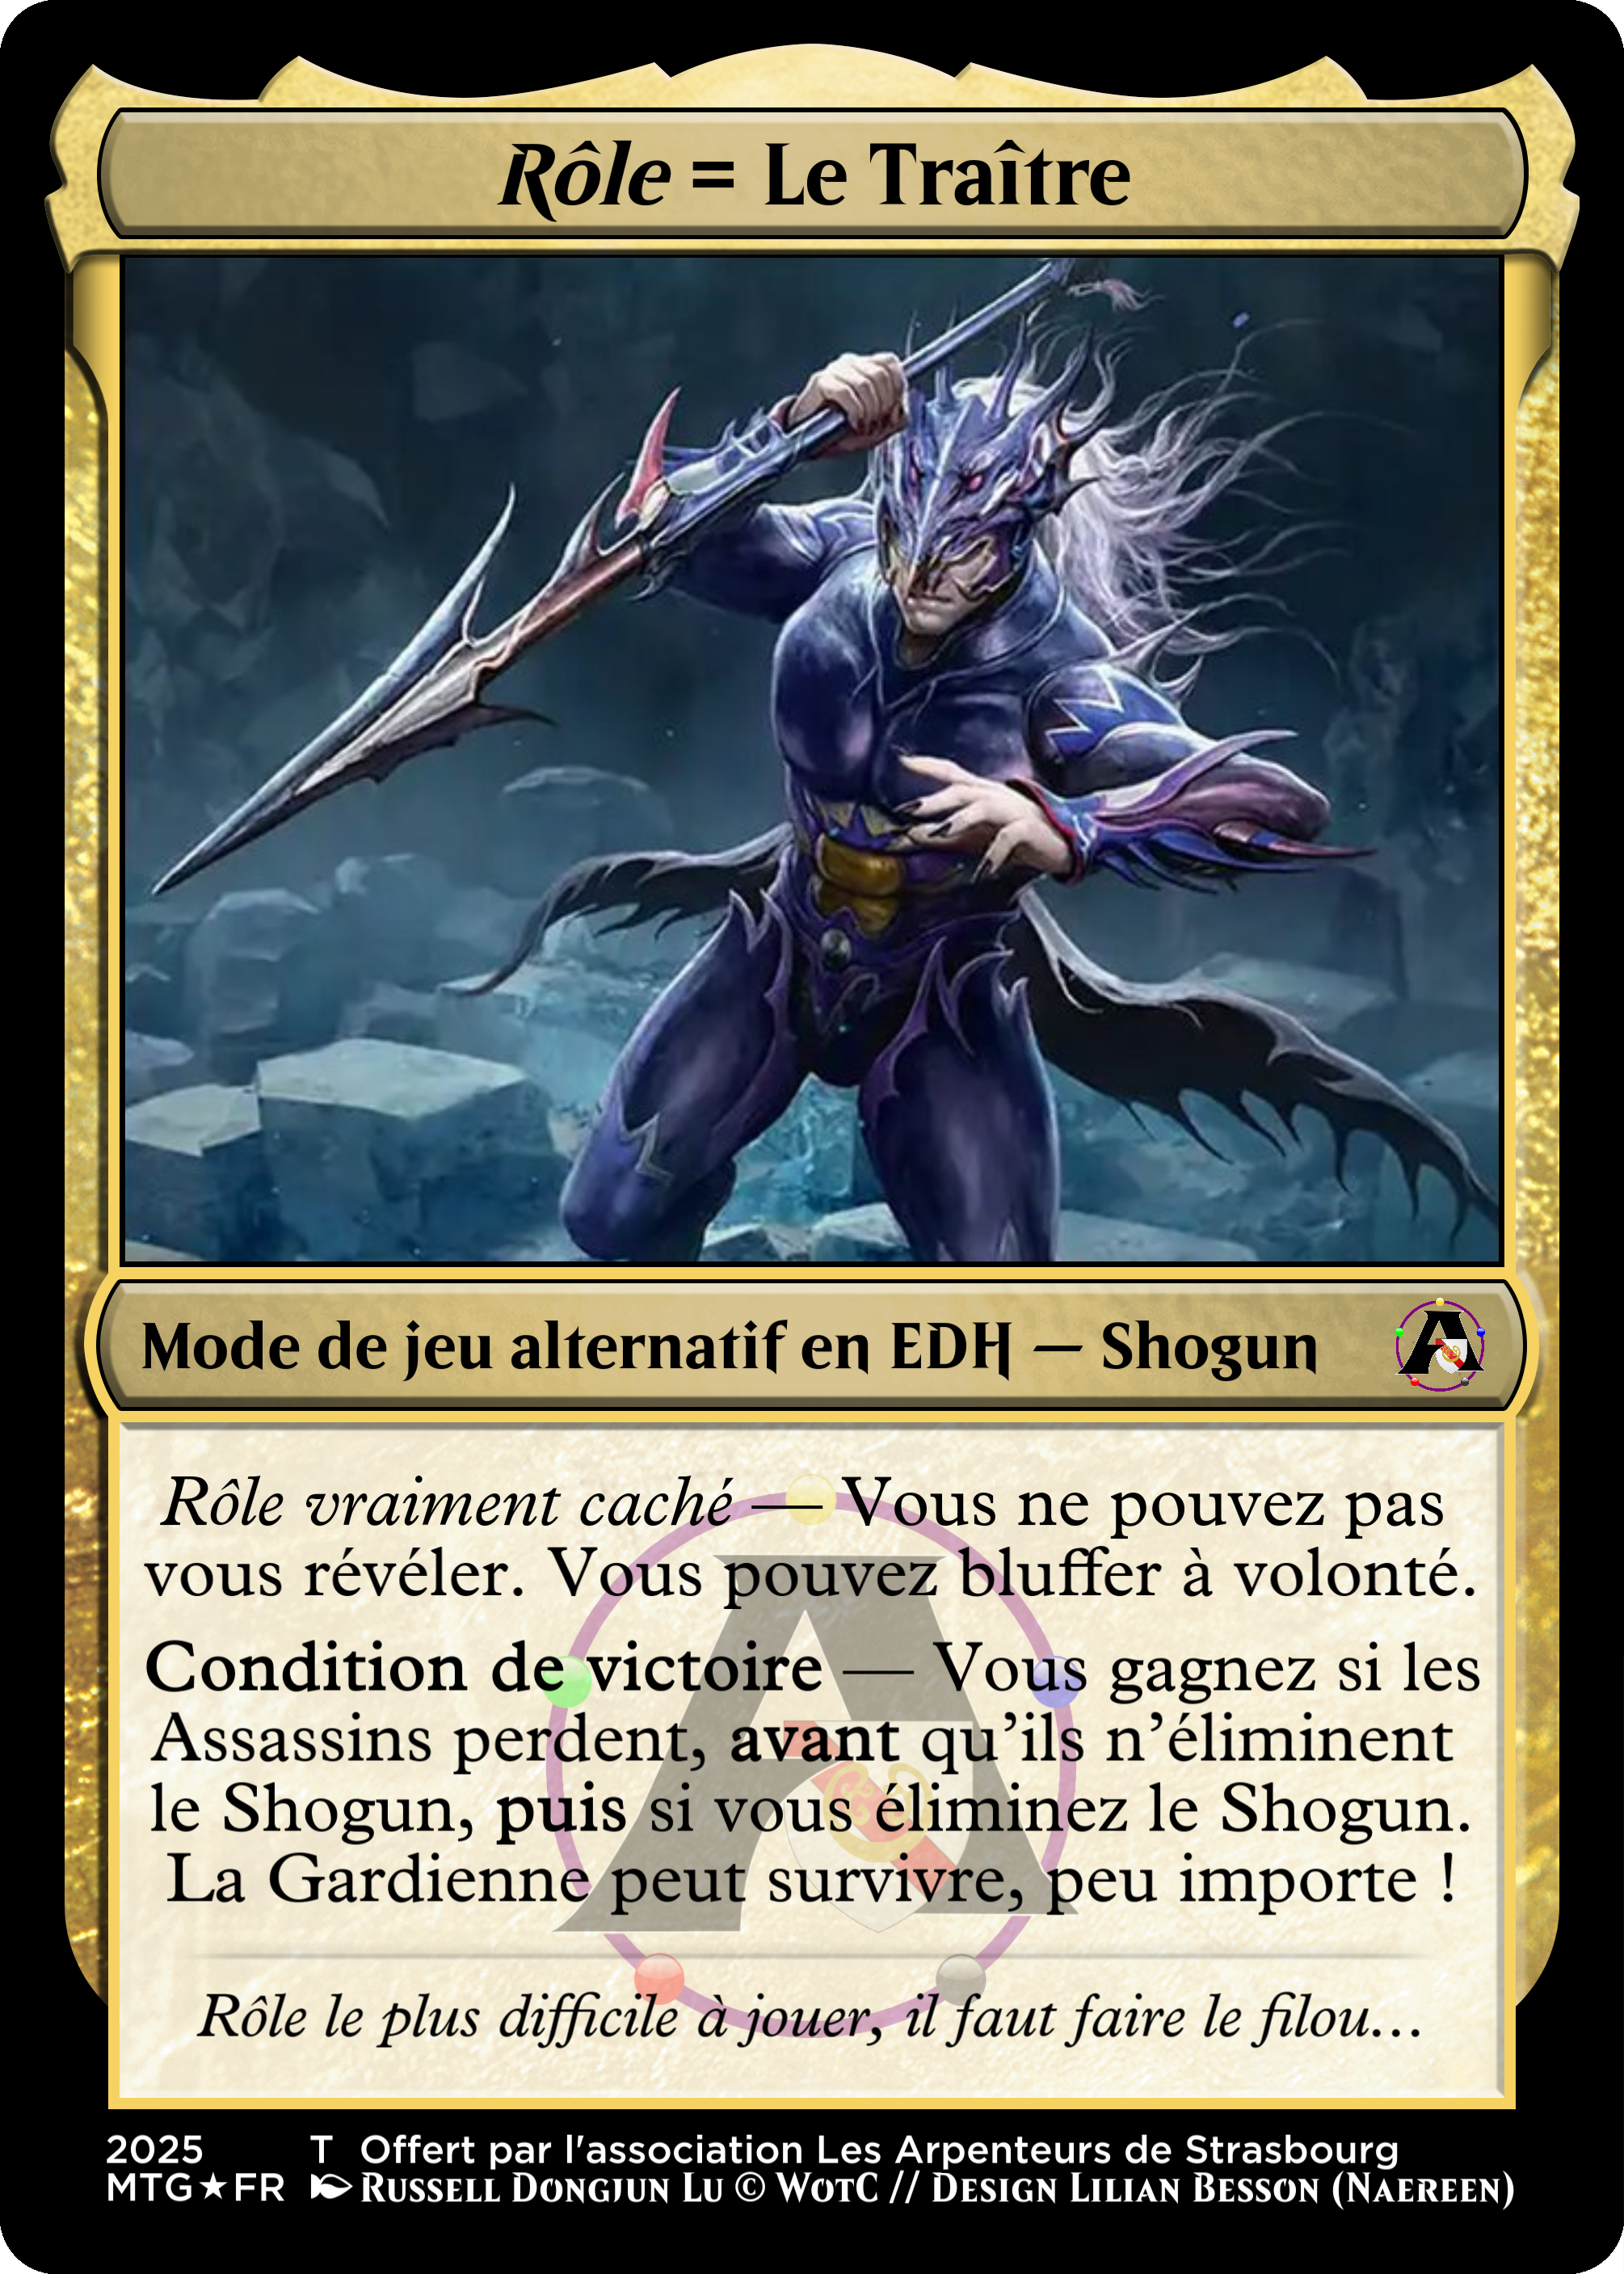
\includegraphics[width=0.21\linewidth]{cartes-pour-le-shogun/traitre.png}
\end{center}

\hfill{}

\subsection*{Avec d'autres variantes ?}

Ce mode de jeu « Shogun » est compatible avec d'autres variantes, comme « Vanguard » ou « Planechase » !
Mais incompatible avec « Treachery ».

% Nous avons déjà testé une partie à quatre joueurs avec « Shogun », « Planechase » \textbf{et} « Shogun », en même temps.
% Cela marche très bien, il faut juste être bien concentré !

\end{document}
